\vfill
\begin{figure}[h!]
    \centering
    \begin{minipage}{.5\linewidth}
        \centering
        \subfloat[Orion Nebula (Messier 42) \cite{orion_nebula_hubble_2006}]{
            \label{:a}
      	  	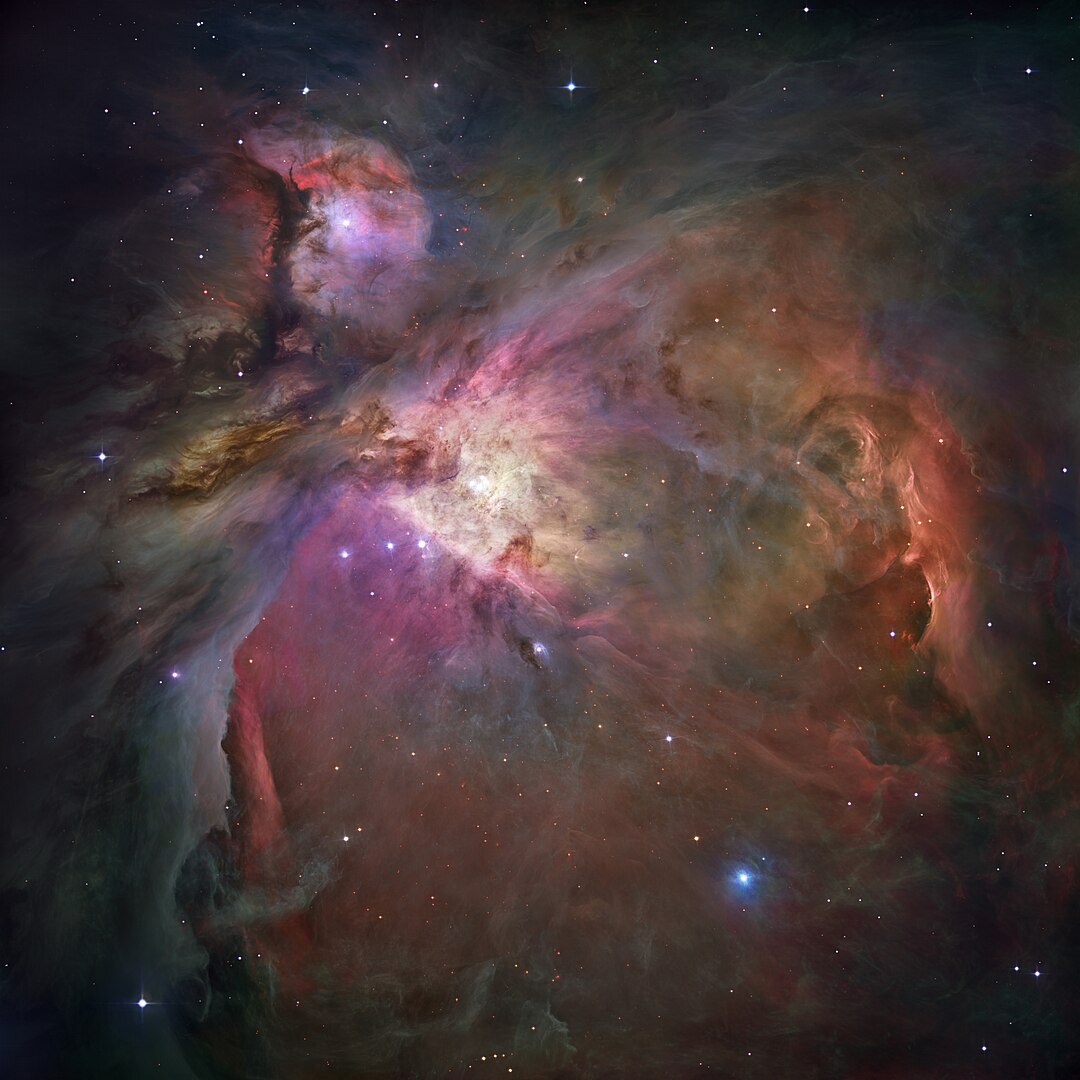
\includegraphics[width=0.85\linewidth]{Orion_Nebula_-_Hubble_2006_mosaic_1080px}
      	}
    \end{minipage}%
    \begin{minipage}{.5\linewidth}
        \centering
        \subfloat[Eagle Nebula (Messier 16) \cite{eagle_nebula_eso_2009}]{
            \label{:b}
            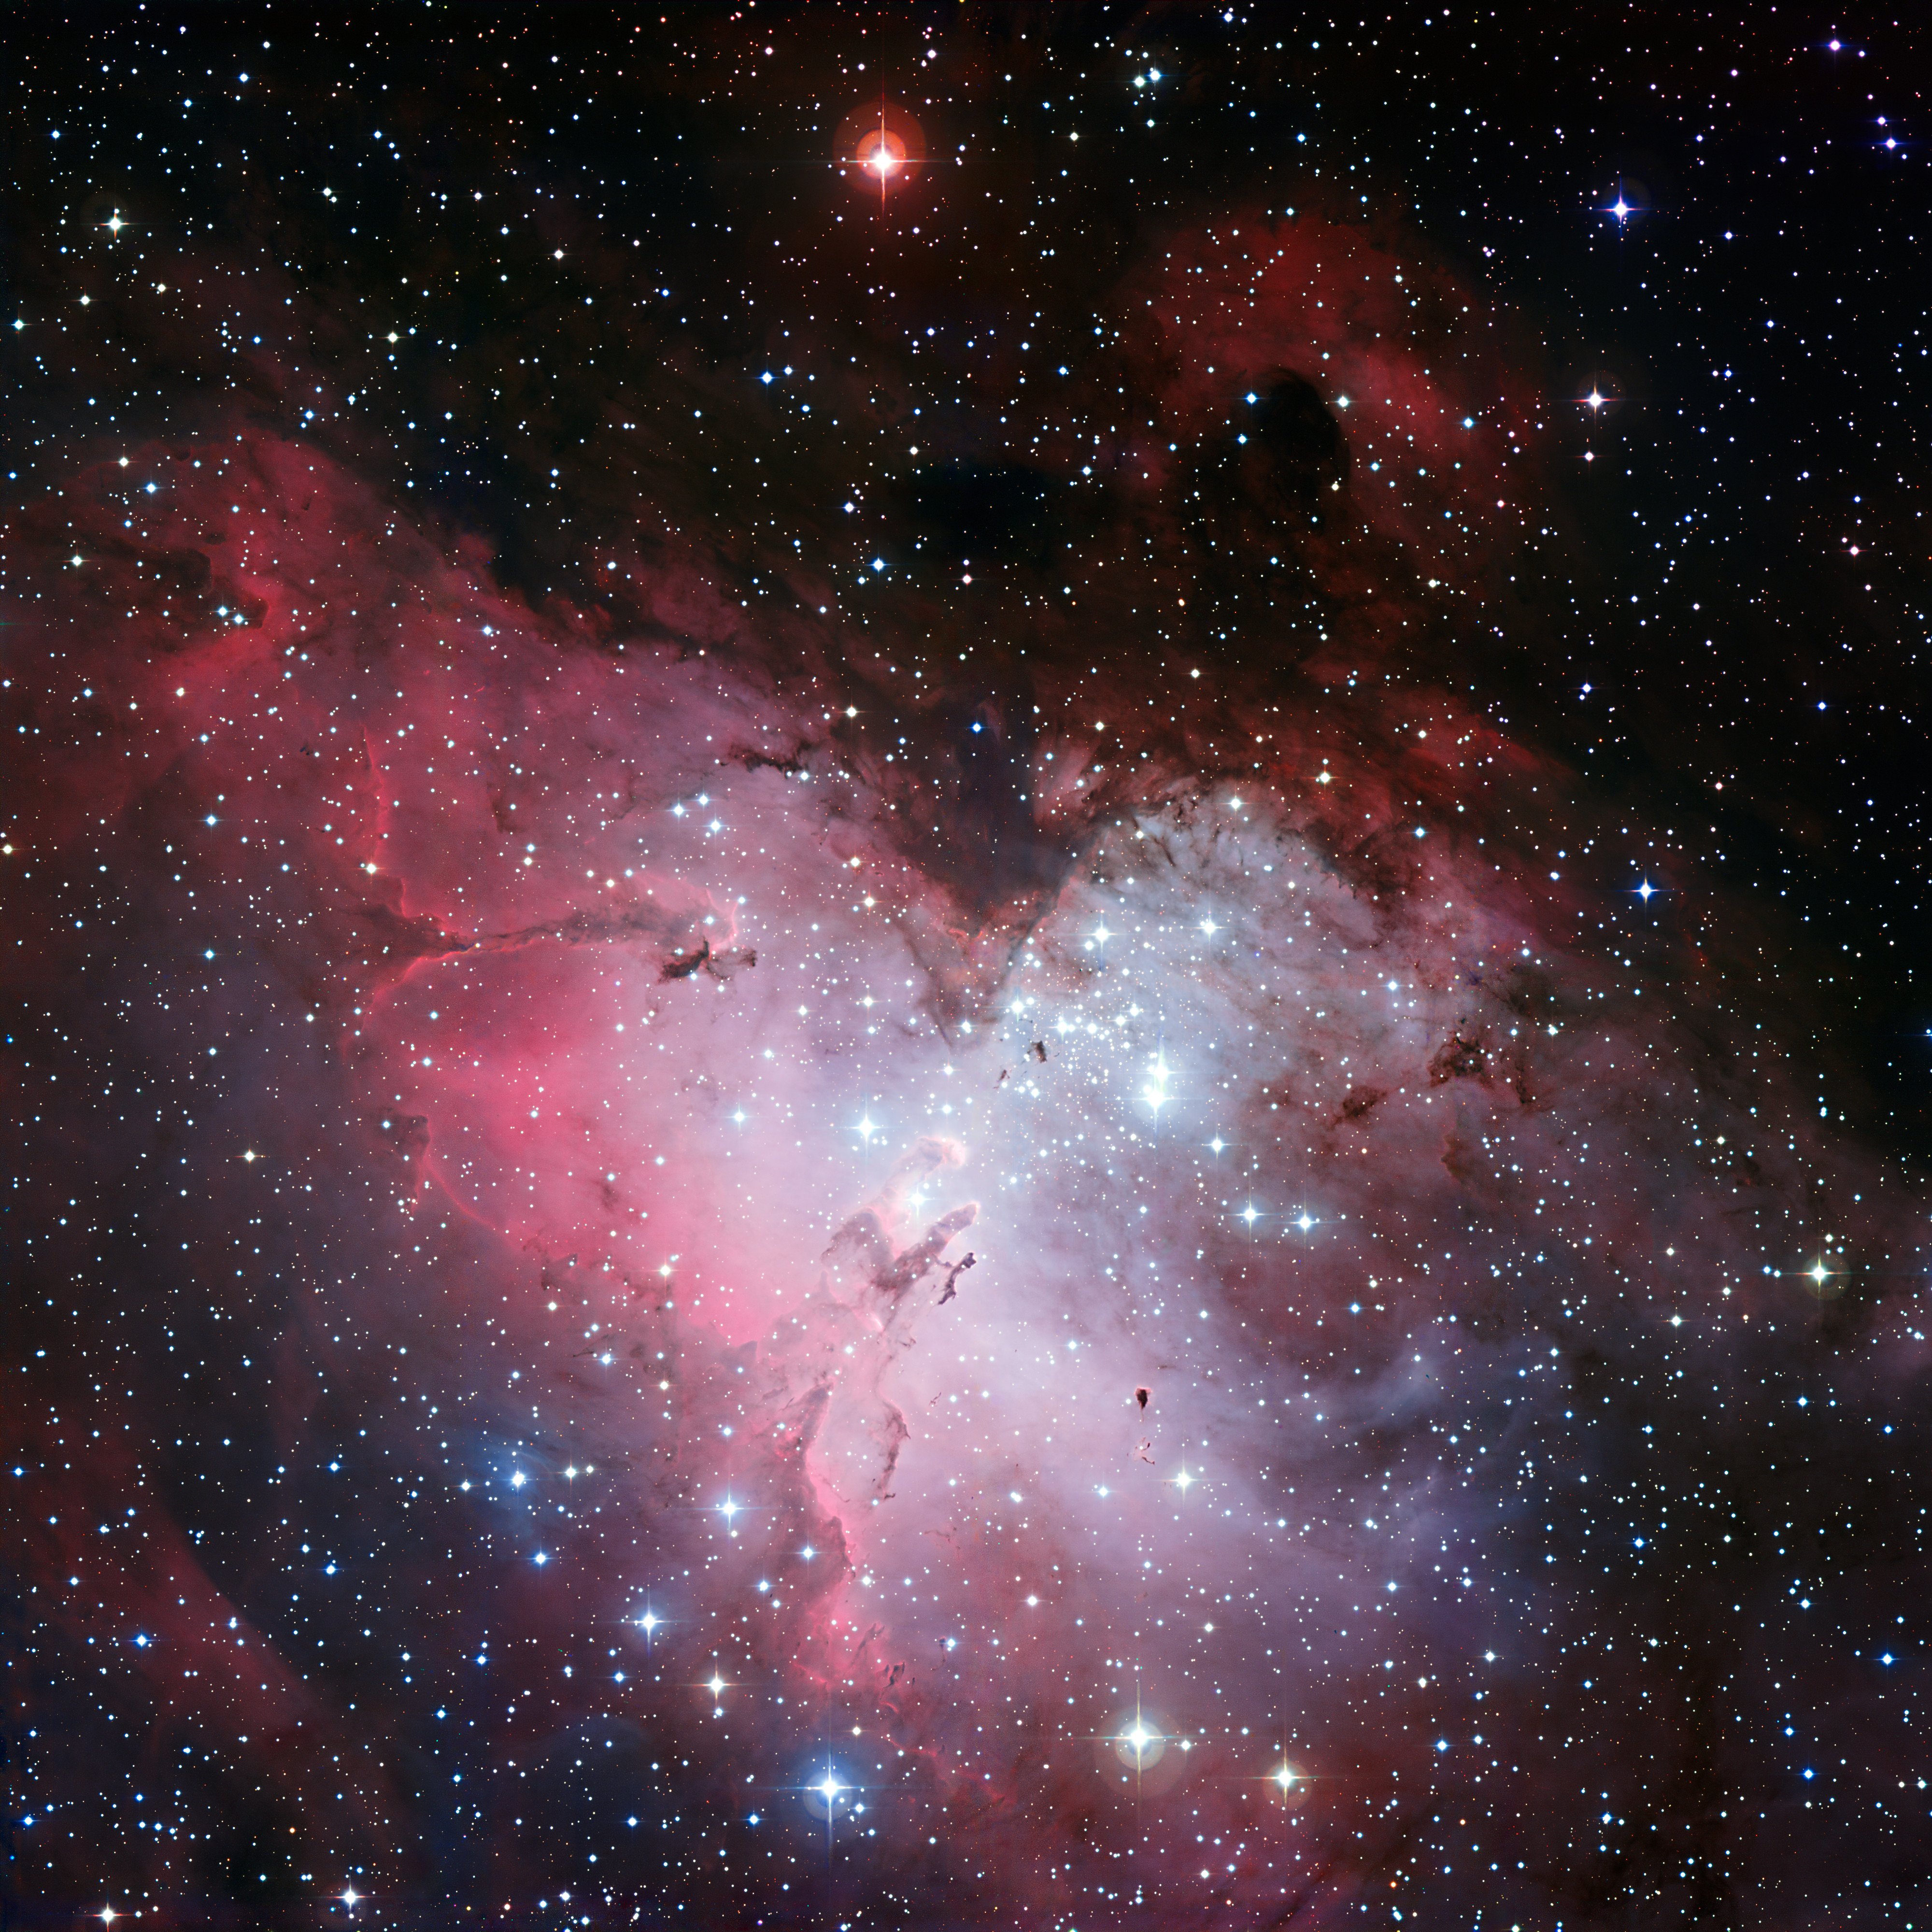
\includegraphics[width=0.85\linewidth]{eso0926a.jpg}
      	}
    \end{minipage}
    \caption{Examples of star-forming regions: (a) The Orion Nebula (b) The Eagle Nebula
        (Zoom in to see the famous \textit{Pillars of Creation} at the center of the image).
    }
    \label{fig:star_forming_regions}
\end{figure}
